\chapter{DUNE Project Management}
\label{ch:detectors-pm}

The international DUNE experiment is managed through two organizations
with highly overlapped personnel: the International DUNE Collaboration
and the International DUNE Project Office. The DUNE Collaboration is
responsible for the scientific and experimental strategy, while the
DUNE Project Office is responsible for the construction of the
experiment in the context of the available international resources.


\section{Overview}

The DUNE project is an international entity that manages
all contributions to the design, construction, installation and
commissioning of the DUNE near and far detectors organized through an
interntional Work Breakdown Structure (WBS). The U.S. DOE-funded
portion of the project, along with all other international
contributions are contained within the DUNE project and its WBS. The DUNE project
will be run as an international project matching DOE project management
requirements. This will imply maintaining a full cost and schedule for
the entire project.  The DOE-funded portion will be managed in a
manner that satisfies DOE requirements and the international
portion will be managed in a similar manner tailored to each
nation's requirements.

The project will directly manage DOE project funds and 
common funds (e.g., construction and operation) collected from the
U.S. and international stakeholders. Unless requested otherwise,
project funding obtained through other agencies will be managed
by groups set up by those agencies.
%However, the entire Project (including international contributions)
%will be subject to the DOE critical decision process incorporating a
%CD-2 baseline cost and schedule approval and a CD-3 start of construction approval.

The DUNE Project will be responsible for monitoring and reporting on
the status of all contributions to the Project, independent of their
funding source, at least to the level of subproject milestones.
Non-DOE partners will report progress to the Project as defined in
formal Memoranda of Understanding (MOU).


\section{DUNE WBS}

The WBS organizes the Project's tasks and deliverables into convienient components. 
This WBS structure is used to organize the cost and schedule for the DUNE project.
The Work Breakdown Structure (WBS) for the International DUNE project is summarized
in this section.

The DUNE Project consists of two major subsystems: the Near Detector (WBS 130.03) and
the Far Detector (WBS 130.05).

The DUNE Near Detector WBS is shown to level 4 in 
%Table~\ref{tab:ND_WBS}
%\begin{table}[ht!]
%\centering
%\begin{tabular}{|l||l|} \hline
%WBS element & Task Name \\ \hline\hline
%{\bf              130.03}  & {\bf Near Detector Systems (NDS)}  \\ \hline
%\hspace{1em}130.03.01      & NDS Conceptual Design        \\ \hline
%\hspace{1em}130.03.02      & NDS Project Management       \\ \hline
%\hspace{2em}130.03.02.01   & NDS Management               \\ \hline
%\hspace{2em}130.03.02.02   & NDS Controls                 \\ \hline
%\hspace{1em}130.03.03      & NDS Beamline Measurements    \\ \hline
%\hspace{1em}130.03.04      & NDS Data Acquisition \& Cmputing    \\ \hline
%\hspace{1em}130.03.05      & Near Neutrino Detector (NND) \\ \hline
%\hspace{2em}130.03.05.01   & NND Management               \\ \hline
%\hspace{2em}130.03.05.02   & NND Magnet                   \\ \hline
%\hspace{2em}130.03.05.03   & NND Electronics              \\ \hline
%\hspace{2em}130.03.05.04   & NND Mechanical               \\ \hline
%\hspace{2em}130.03.05.05   & NND Assembly, Installation \& Test  \\ \hline
%\hspace{2em}130.03.05.06   & NND DAQ                      \\ \hline
%\end{tabular}
%\caption{DUNE Near Detector Breakdown Structure (WBS) shown at L4.}
%\label{tab:ND_WBS}
%\end{table}
%and is shown graphically in 
Fig.~\ref{fig:ND_WBS}.
\begin{cdrfigure}[Near Detector WBS]{ND_WBS}{Near Detector Work Breakdown Structure.}
\centering
\begin{center}
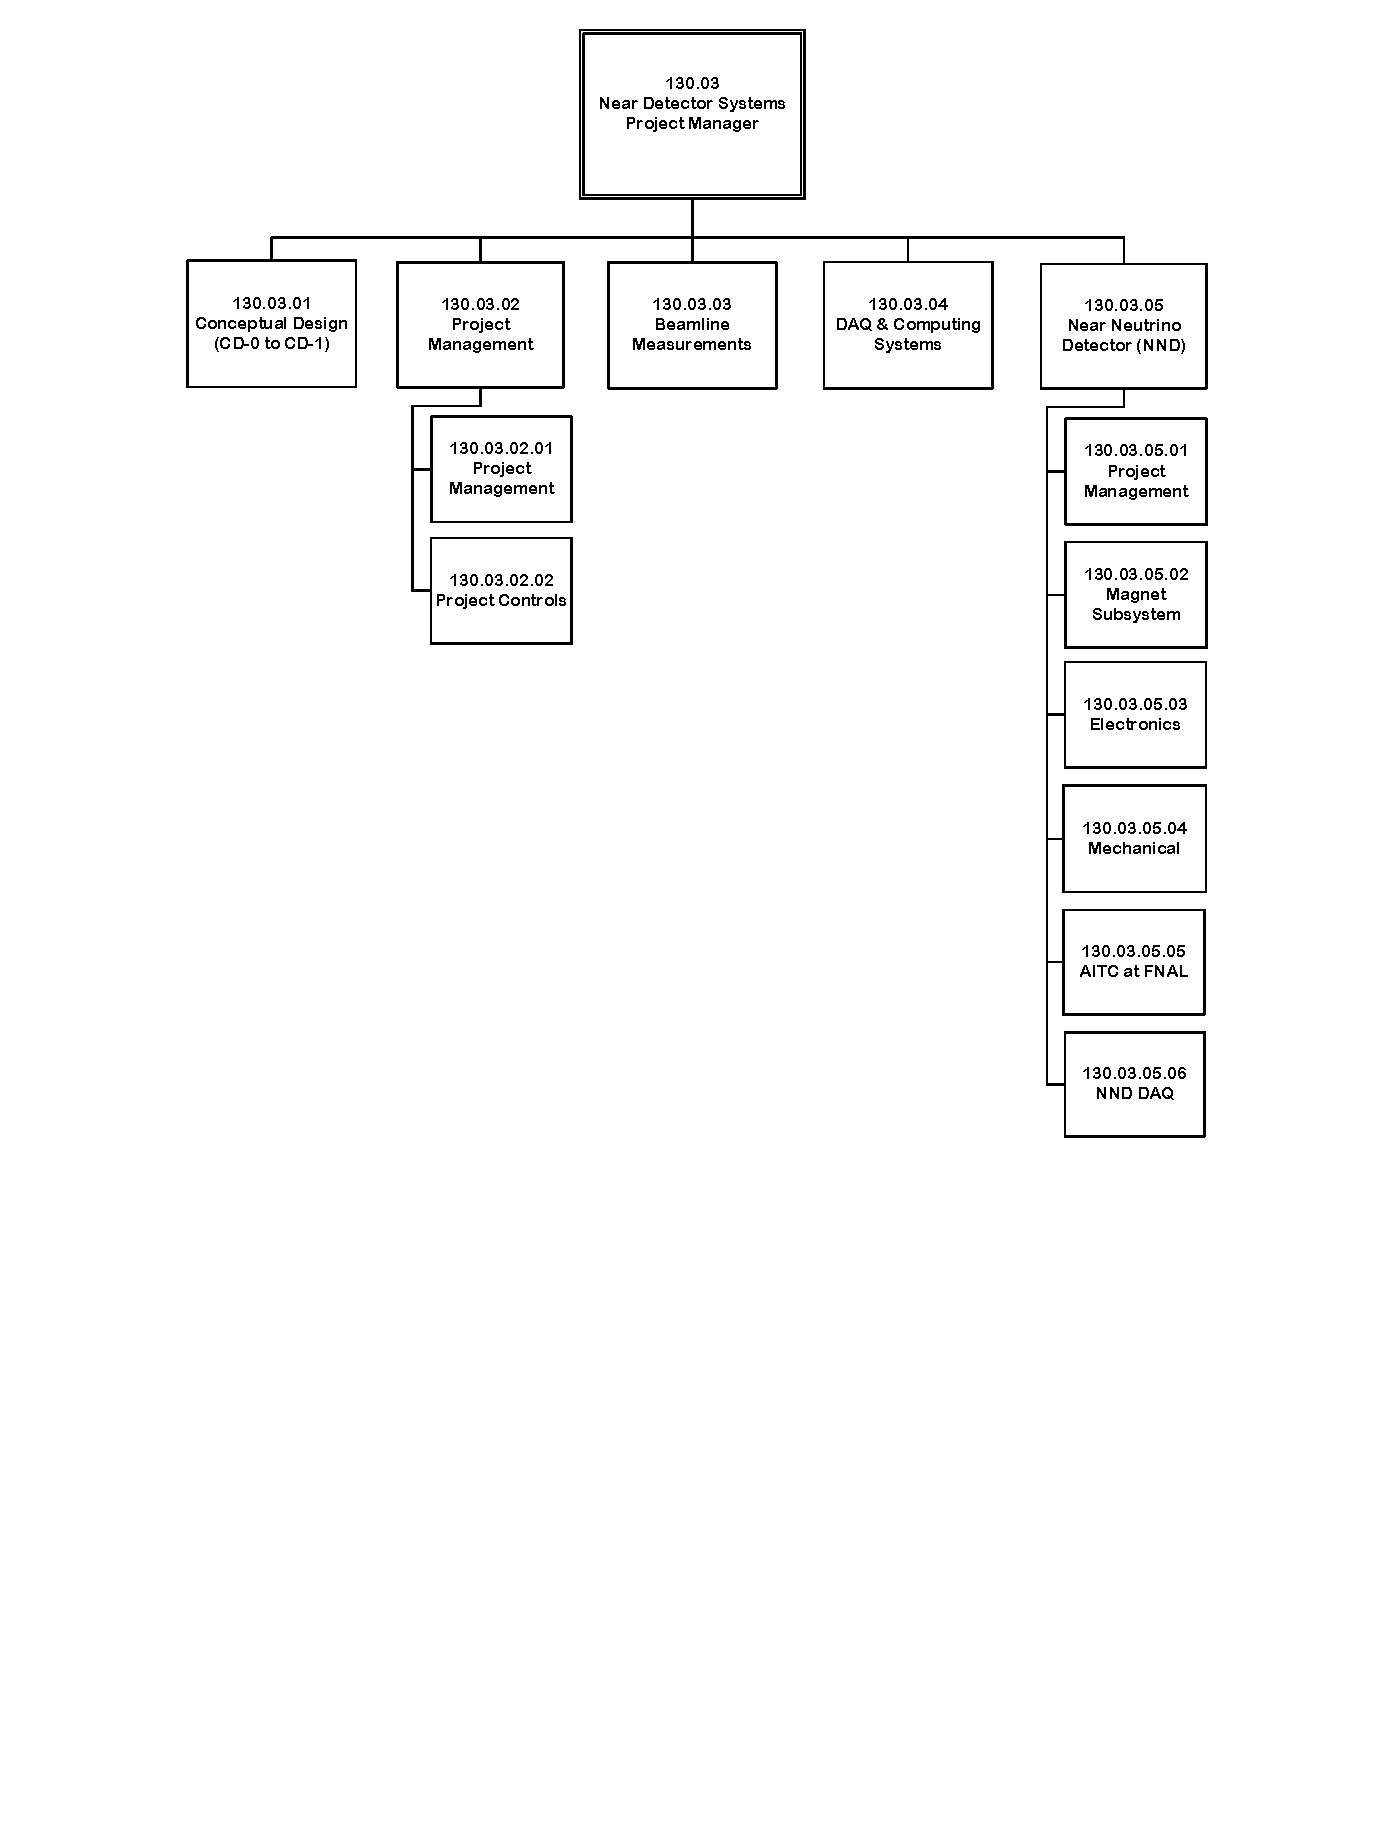
\includegraphics[width=1.\textwidth]{ND_documents_nonames.pdf}
\end{center}
\end{cdrfigure}
The DUNE Far Detector WBS is shown to level 3 in 
%Table~\ref{tab:FD_WBS}
%\begin{table}[ht!]
%\centering
%\begin{tabular}{|l||l|} \hline
%WBS element & Task Name \\ \hline\hline
%{\bf               130.05} & {\bf Far Detector}           \\ \hline
%\hspace{1em}130.05.01      & Management                   \\ \hline
%\hspace{1em}130.05.02      & Time Projection Chamber      \\ \hline
%\hspace{1em}130.05.03      & DAQ \& Monitoring            \\ \hline
%\hspace{1em}130.05.04      & Installation \& Commissioning  \\ \hline
%\hspace{1em}130.05.05      & Photon Detector              \\ \hline
%\hspace{1em}130.05.06      & Cold Electronics             \\ \hline
%\end{tabular}
%\caption{DUNE Far Detector Breakdown Structure (WBS) shown at L3.}
%\label{tab:FD_WBS}
%\end{table}
%and is shown graphically in 
Fig.~\ref{fig:FD_WBS}.
\begin{cdrfigure}[Far Detector WBS]{FD_WBS}{Far Detector Work Breakdown Structure.}
\centering
\begin{center}
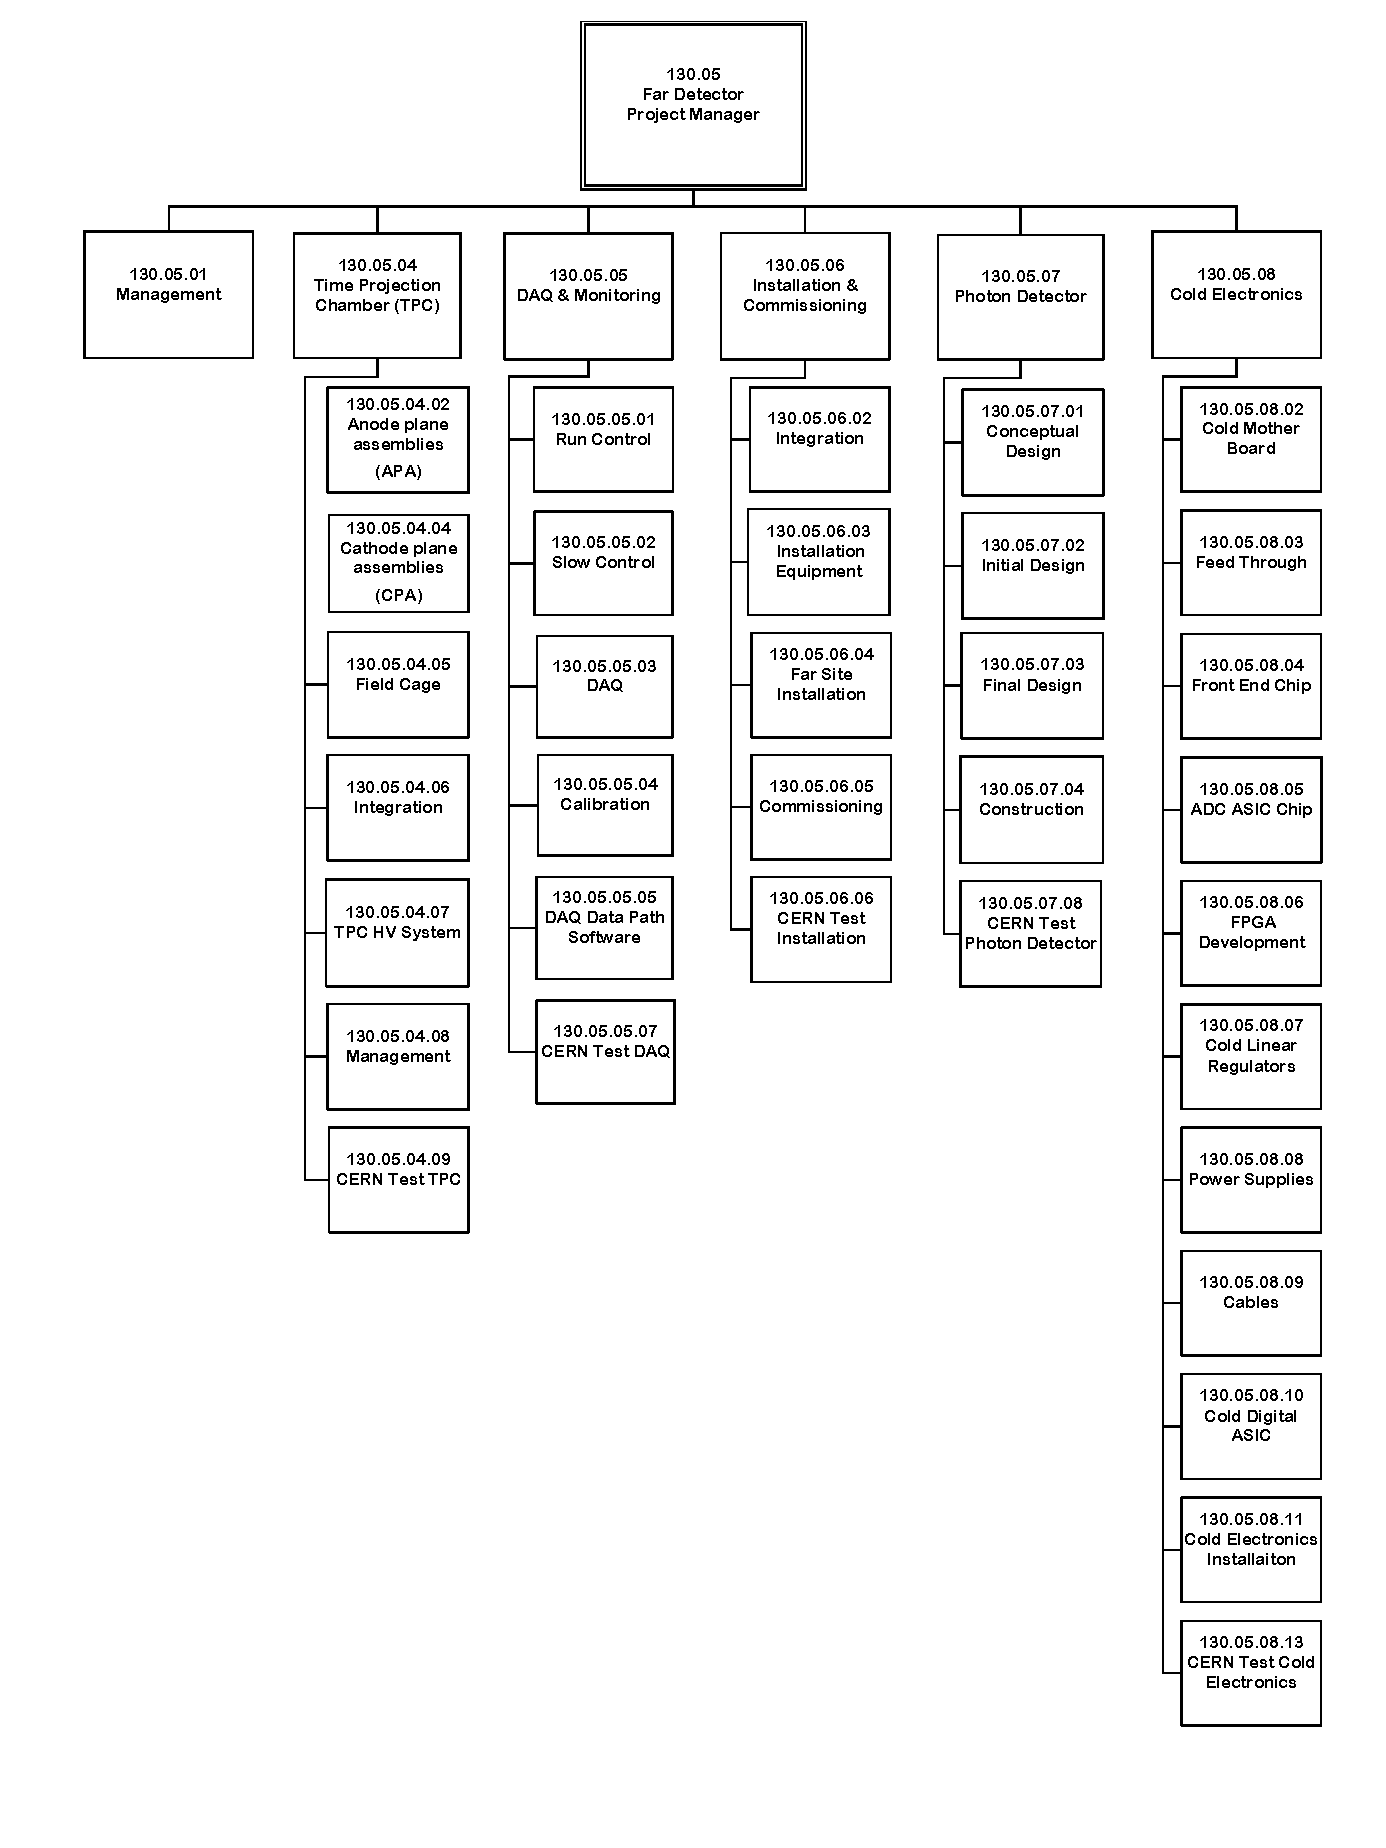
\includegraphics[width=1.\textwidth]{FD_documents_nonames.pdf}
\end{center}
\end{cdrfigure}

The DUNE project organization and structure will evolve as the project
becomes more fully internationalized.
